\subsubsection{DC- og AC-kretser}
\paragraph{Kondensator i DC-kretser} \mbox{} \\
En kondensator i en DC krets vil bli ladet opp
til det elektriske feltet i kondensatoren kansellerer effekten av
det elektriske feltet i spenningskilden.
Da vil det ikke gå noe strøm lenger.

\paragraph{Kondensator i AC-kretser} \mbox{} \\
Strømmen I gjennom en kondensator er proporsjonal med forandring i spenning.
$$I = C \cdot \frac{dV}{dt}$$
Det vil si at det går mer strøm når spenning forandrer seg mest. \\
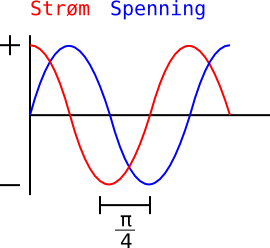
\includegraphics[width=0.5\textwidth]{./img/kondensator-spenning} \\
Vi ser at strømmen er størst når spenningen er 0.
Det er fordi strømmen er gitt ved den derivert av spenning,
og den største forandring i spenning er ved 0.
\\\\
Husk at {\color{green} effekt (P)} er gitt ved $P = U \cdot I$. \\
Vi ser forholdet mellom strøm, spenning og effekt. \\
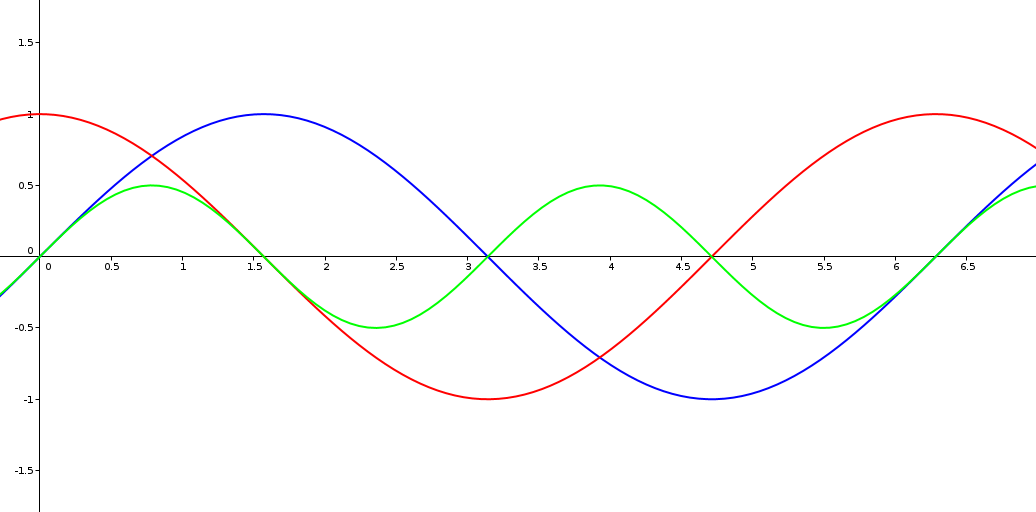
\includegraphics[width=\textwidth]{./img/kondensator-power} \\



\subsubsection{Reaktanse}
Når en kondensator er i en AC-krets fungerer den som en motstand.
Vi kaller denne motstanden reaktans ($X_C$).
Reaktans er gitt ved
$$X_C = \frac{1}{2 \pi f C}$$
f = frekvens \\
C = kapasitet
\\\\
Vi ser fra dette at motstanden i en kondensator
minker når frekvensen øker.



\paragraph{Serie- og parallellkobling} \mbox{} \\
Koblinger med hensyn på reaktans fungerer som med motstander.
\\\\
Seriekobling
$$X_{CT} = X_{C1} + ... + X_{Cn}$$
Parallellkobling
$$\frac{1}{X_{CT}} = \frac{1}{X_{C1}} + ... + \frac{1}{C_{Cn}}$$




\subsubsection{RC-kretser}
Impedans \\
TODO
